\documentclass[]{article}
\usepackage[a4paper, total={6in, 10in}]{geometry}
\usepackage{hyperref}
\usepackage{amsmath}
\usepackage{graphicx}
\usepackage[outdir=./]{epstopdf}
\usepackage{booktabs}
\usepackage{float}
\usepackage{subcaption}

\setlength{\parindent}{0em}
\setlength{\parskip}{1em}

\DeclareMathOperator{\cov}{cov}

%opening
\title{SSY 230, System Identification\\
	Project 3: Identification of a Real System}
\author{Yuxuan Xia\\ \href{mailto:yuxuan.xia@chalmers.se}{yuxuan.xia@chalmers.se}\\Emil Staf\\\href{mailto:emil.staf@chalmers.se}{emil.staf@chalmers.se}}

\begin{document}

\maketitle


\section{Flexible Robot Arm}
The system we have chosen to identify is a mechanical system, where a flexible robot arm have been installed on an electrcal motor. It is a SISO system where the input $u(t)$ is measured reaction torque and the output $y(t)$ is the acceleration of the flexible robot arm. The experimental set-up was performed using a periodic sinusodial sweep.

\subsection{Data}
As mentioned previously the input data is a periodic sinusodial sweep (see top plot of Figure \ref{fig:input}). Due to the fact that the data was obtained using a periodic sinusodial sweep we split the data in half and use the first part as training data and the second part as validation data.

\begin{figure}[ht]
\centering
\includegraphics[trim= 10cm 8cm 10cm 8cm, scale=0.4]{figures/input.pdf}
\caption{System data, input $u(t)$ (top) and output $y(t)$ (bottom).}
\label{fig:input}

\end{figure}
To make sure that the frequency content in both the training and validation data are similar we use the \emph{etfe} in MATLAB to find the Empirical Transfer Function Estimate of training- and validation data. The resulting bode-plot is shown in Figure \ref{fig:bode-train_valid}.

\begin{figure}[ht]
\centering
\begin{subfigure}{.49\textwidth}
	\centering
	\includegraphics[trim= 10cm 8cm 10cm 8cm, scale=0.4]{figures/bode-train_valid.pdf}
	\caption{Bode-plot of training and validation data.}
	\label{fig:bode-train_valid}
\end{subfigure}
\begin{subfigure}{.49\textwidth}
	\centering
	\includegraphics[trim= 10cm 8cm 10cm 8cm, scale=0.4]{figures/periodogram-train_valid.pdf}
	\caption{Periodogram of training and validation data.}
	\label{fig:periodogram-train_valid}
\end{subfigure}
\caption{Analyzing training/validation split.}
\label{fig:train_valid}
\end{figure}

From analysing Figure \ref{fig:bode-train_valid} it is clear that the amplitude of the frequency content in both training- and validation data is very similar, while there is a 360 degree phase shift approximately starting from frequencies $>0.35$ rad/s. However, it should be noted that a 360 degree phase shift means the validation data and training data are still in phase. Using the MATLAB build-in function \emph{periodogram} it is clear that the frequency content of the training- and validation data is very similar. Also, it can be seen that for frequencies $> 0.5$ rad/s the power the amount of information for each frequency decreases. By examining the bode plot, we can have an initial guess of the number of poles and zeros we can observe that there are four sharp corners, each of which represent two conjugate poles or two conjugate zeros depending on its concave or convex. The first and last parts of the amplitude plot are ladder-shaped, which means that there are two more real poles. And we can also see that there is one hollow between two spikes, which represent a zero. Thus, there are six poles and five zeros in total. The high frequency assymptote amplitude is constant, which means that (for a linear system) there should be an equal amount of poles and zeroes.

\subsection{Pre-Processing}
...

\subsection{Model Estimation}
\subsubsection{Linear Models}
 In this section we search over the linear model space for candidate models. A few different linear models are tested and compared: ARX, OE, State Space and Transfer Function Estimation. 

\begin{figure}[ht]
\centering
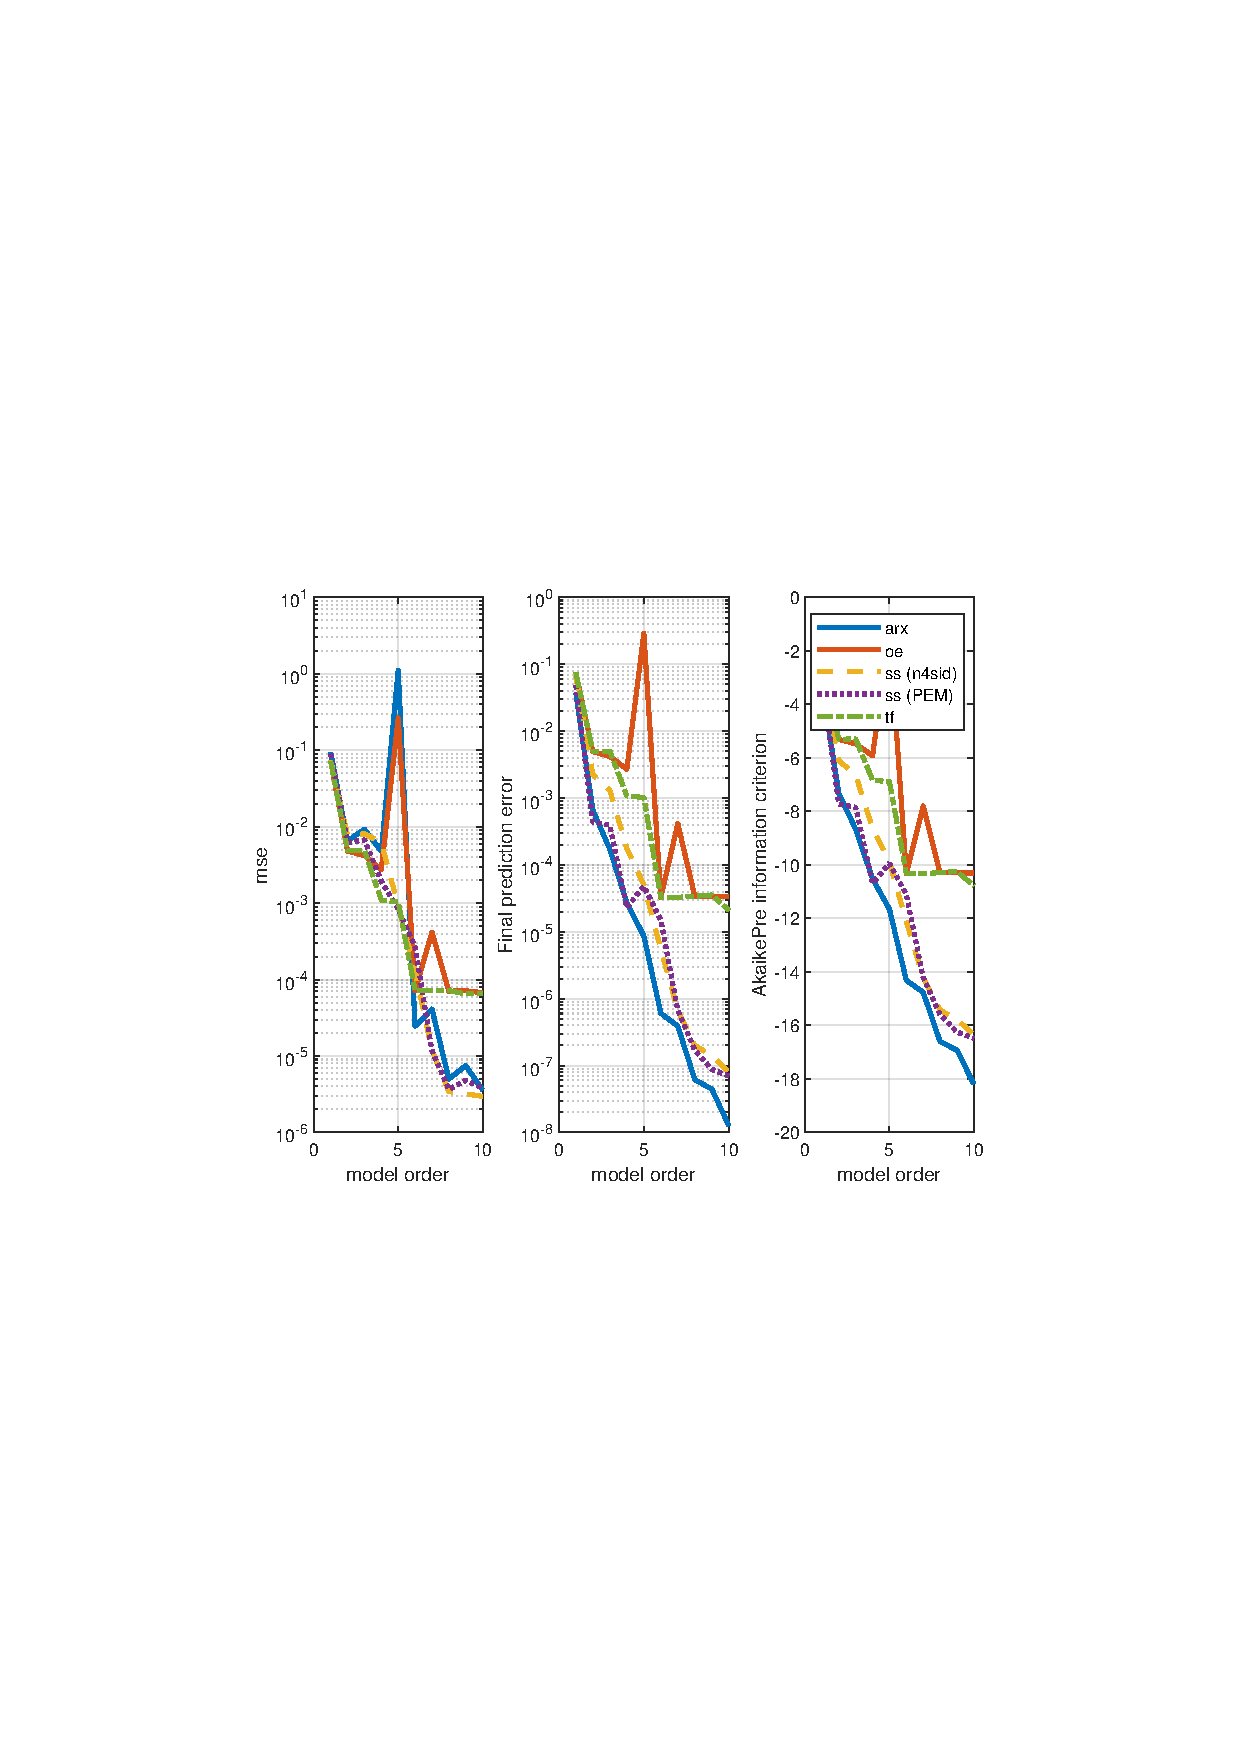
\includegraphics[trim= 10cm 8cm 10cm 8cm, scale=0.7]{figures/model_order.pdf}
\caption{Searching over different model orders $n$, where the number of parameters $p$ are $p=2n+1$.}
\label{fig:model_order}
\end{figure}
In Figure \ref{fig:model_order} the $mse$ decreases for increasing model order but start to saturate for model orders above 8. As the high frequency assymptote from the bode plot of the ETFE tells us that there should be an equal ammount of poles and zeroes, and our more specific analysis resulted in 6 poles and 5 zeroes we first try models of order 6. From Figure \ref{fig:model_order} the $mse$ shows that the models ARX, and State Space give the best results so lets focus on analysing them from now on.

\paragraph{Pole-Zero Plots}
\begin{figure}[ht]
\centering
\begin{subfigure}{.49\textwidth}
	\centering
	\includegraphics[trim= 10cm 8cm 10cm 8cm, scale=0.4]{figures/pz_arx_66.pdf}
	\caption{ARX na = 6 nb=6.}
	\label{fig:pzplot_arx1}
\end{subfigure}
\begin{subfigure}{.49\textwidth}
	\centering
	\includegraphics[trim= 10cm 8cm 10cm 8cm, scale=0.4]{figures/pz_arx_65.pdf}
	\caption{ARX na=6 nb=5.}
	\label{fig:pzplot_arx2}
\end{subfigure}
\end{figure}


\begin{figure}[ht]
\centering
\includegraphics[trim= 10cm 8cm 10cm 8cm, scale=0.7]{figures/pz_n4sid_66.pdf}
\caption{State Space ($n4sid$).}
\label{fig:pzplot_ss}
\end{figure}

\begin{figure}[ht]
\centering
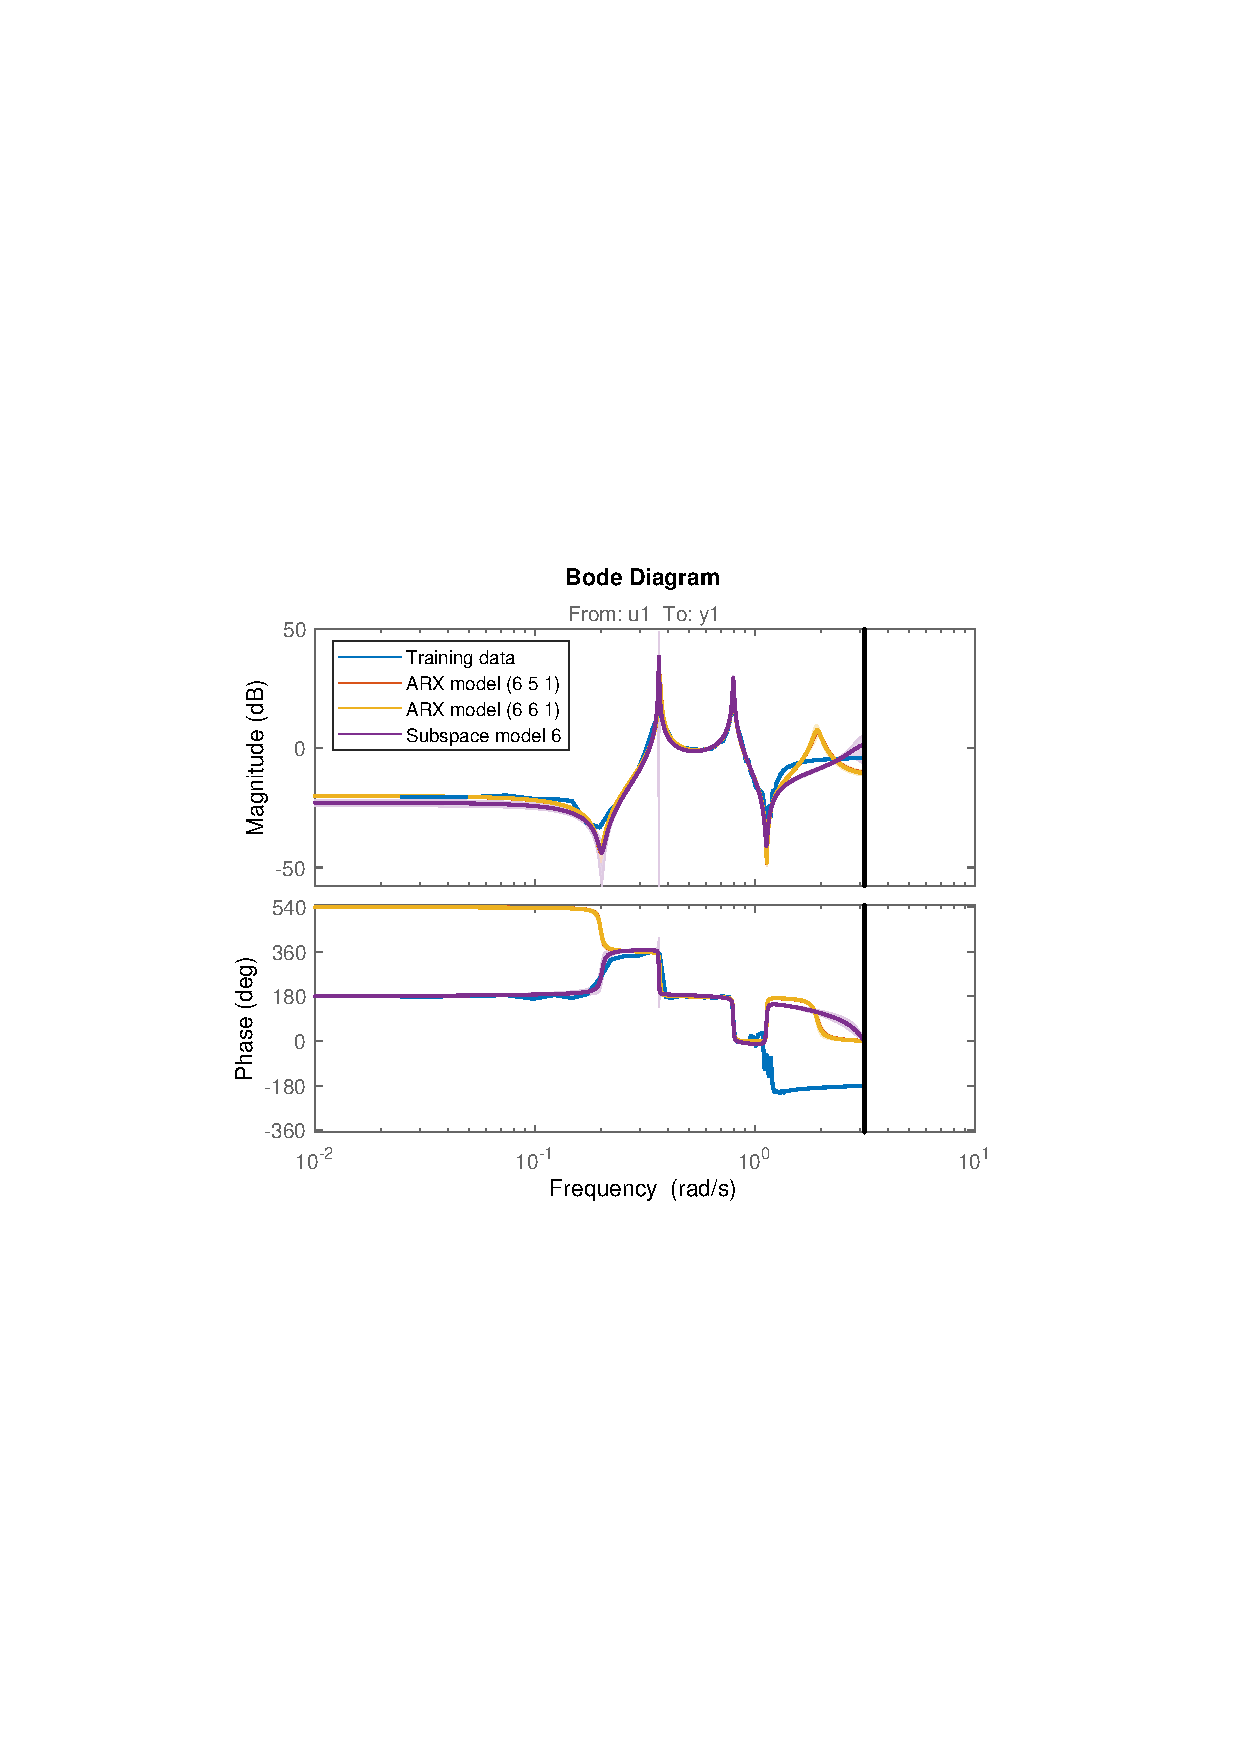
\includegraphics[trim= 10cm 8cm 10cm 8cm, scale=0.7]{figures/bode_models.pdf}
\caption{Bode plot of models.}
\label{fig:bode_models}
\end{figure}
In Figure \ref{fig:bode_models}, we can see that the gain margin when phase is at -180 degree, around the Nyquist frequency varies a lot compared to the empirical transfer function update, which is almost constant. This implies that we probability need some further data preprocessing step to filter out the high frequency component of the data.


\paragraph{Simulations}

\paragraph{Pole-Zero Plots}
\begin{figure}[ht]
\centering
\begin{subfigure}{.49\textwidth}
	\centering
	\includegraphics[trim= 10cm 8cm 10cm 8cm, scale=0.4]{figures/simulations.pdf}
\end{subfigure}
\begin{subfigure}{.49\textwidth}
	\centering
	\includegraphics[trim= 10cm 8cm 10cm 8cm, scale=0.4]{figures/sim_diff_arx_ss.pdf}
\end{subfigure}
\caption{Simulations (left) and simulation error comparison of ARX and State Space model (right).}
\label{fig:simulations}
\end{figure}

\begin{figure}[ht]
\centering
\includegraphics[trim= 10cm 8cm 10cm 8cm, scale=0.7]{figures/sim_diff_matrix.pdf}
\caption{Model differences and simulation vs validation data error on diagonal.}
\label{fig:model_differences_simulation}
\end{figure}

\paragraph{Predictions}

\paragraph{Pole-Zero Plots}
\begin{figure}[ht]
\centering
\begin{subfigure}{.49\textwidth}
	\centering
	\includegraphics[trim= 10cm 8cm 10cm 8cm, scale=0.4]{figures/predictions.pdf}
\end{subfigure}
\begin{subfigure}{.49\textwidth}
	\centering
	\includegraphics[trim= 10cm 8cm 10cm 8cm, scale=0.4]{figures/pred_diff_arx_ss.pdf}
\end{subfigure}
\caption{Predictions (left) and prediction error comparison of ARX and State Space model (right).}
\label{fig:predictions}
\end{figure}

\begin{figure}[ht]
\centering
\includegraphics[trim= 10cm 8cm 10cm 8cm, scale=0.7]{figures/pred_diff_matrix.pdf}
\caption{Model differences and prediction vs validation data error on diagonal.}
\label{fig:model_differences_prediction}
\end{figure}

\paragraph{correlations}
\begin{figure}[ht]
\centering
\begin{subfigure}{.49\textwidth}
	\centering
	\includegraphics[trim= 10cm 8cm 10cm 8cm, scale=0.4]{figures/auto-corr-1step.pdf}
\end{subfigure}
\begin{subfigure}{.49\textwidth}
	\centering
	\includegraphics[trim= 10cm 8cm 10cm 8cm, scale=0.4]{figures/cross-corr-1step.pdf}
\end{subfigure}
\caption{Auto-Correlation (left) and cross-correlation (right).}
\label{fig:correlations}
\end{figure}

\subsubsection{Non-linear models}
\begin{figure}[ht]
\centering
\begin{subfigure}{.49\textwidth}
	\centering
	\includegraphics[trim= 10cm 8cm 10cm 8cm, scale=0.4]{figures/predictions_nl.pdf}
\end{subfigure}
\begin{subfigure}{.49\textwidth}
	\centering
	\includegraphics[trim= 10cm 8cm 10cm 8cm, scale=0.4]{figures/simulations_nl.pdf}
\end{subfigure}
\caption{Non-linear model predictions (left) and simulations (right).}
\label{fig:correlations}
\end{figure}

\end{document}
